%!TEX root = main.tex

\vspace{-0.5em}
\paragraph*{Problem Setting}
Assume a set of real numbers $\Omega = \{x_1, \ldots, x_N\}$ 
with cardinality $N$, where $x_1 \leq x_2 \leq \ldots \leq x_N$.
W.l.o.g, assume 
that all real numbers in $\Omega$ are 
in $[0, 1]$. 

The goal is to find an partition $\setI = \{I_j\}_{j = 1}^k$ of $[0, 1]$ into $k$ disjoint intervals, so that if we quantize every $x \in I_j$ to an endpoint of $I_j$, the variance is minimal over all possible partitions of $[0, 1]$ into $k$ intervals.
Formally:
\begin{align}
\nonumber \min_{\setI: |\setI| = s} \quad & \mathcal{MV}(\setI) := {1\over N}\sum_{j = 1}^k \sum_{x_i \in I_j} \err(x_i, I_j)\\
\text{s.t.}\quad & \bigcup_{j = 1}^k I_j = [0, 1],
\label{eq:opt_Q}
\end{align}
where $\err (x, I) = (b - x) (x - a)$ is the variance for point $x \in I$ if we quantize $x$ to an endpoint of $I = [a, b]$.
That is, $\err (x, I)$ is the variance of the (unique) distribution $D$ supported on ${a, b}$  so that $\E_{X \sim D} [X] = x$.

%\begin{align}
%\nonumber \min_{l_1, \cdots, l_{s-1}} \quad & \mathcal{MV}(l_1,\cdots, l_{s-1}) := {1\over N}\sum_{x\in \Omega} \sum_{k=1}^s {\bf 1}_k(x)V_k(x)\\
%\text{s.t.}\quad & 0 = l_0 \leq l_1\leq l_2 \leq \cdots \leq l_{s-1} \leq l_s = 1.
%\label{eq:opt_Q}
%\end{align}

Given an interval $I \subseteq [0, 1]$, we let $\setX_I$ be the set of $x_j \in \setX$ contained in $I$.
We also define $\err (\setX, I) = \sum_{x_j \in I} \err (x_j, I)$.
Given a partition $\setI$ of $[0, 1]$, we let $\err (\setX, \setI) = \sum_{I \in \setI} \err (\setX, I)$.
We also let the optimum solution be $\setI^* = \argmin_{|\setI| = k} \err (\setX, \setI)$ (randomly break the tie), and we let $\OPT_k = \err(\setX, \setI^*)$.


\vspace{-0.5em}
\subsection{Dynamic Programming}
\vspace{-0.5em}

We first present a dynamic programming algorithm
that solves the above problem in an exact way.
In the next subsection, we present a more practical
approximation algorithm that only needs to scan all
data point once.

One challenging to solve this problem is 
due to non-convexity and non-smoothness. 
Our algorithm is based on the observation that
there exists an optimal solution which places endpoints at input points. We have

\begin{lemma}
\label{lem:discrete}
There is a $\setI^*$ so that all endpoints of any $I \in \setI^*$ are in $\Omega \cup \{0, 1\}$.
\end{lemma}


\iffalse
\begin{proof}
Fix any endpoint $b$ of intervals in $\setI^*$.
WLOG assume that $b \neq 0, 1$.
Then we must have $I = [a, b]$ and $I' = [b, c]$ for some $I, I' \in \setI^*$.
Observe that the choice of $b$ only affects the error for points in $I \cup I'$.
We have that $\err (\Omega, I) + \err (\Omega, I') $ is given by
\begin{align*}
& \sum_{x \in I} (b - x) (x - a) + \sum_{x \in I'} (c -x)(x - b) \\
&= A b + C \; ,
\end{align*}
where $A, C$ are constants which do not depend on $b$.
Hence, this is a linear objective in $b$.
Since $b$ can freely range between the rightmost point in $I$ and the leftmost point in $I'$, there is an optimizer for this solution at one of those two points.
Hence we may choose $b \in \Omega$.
\end{proof}
\fi


Therefore, to solve the problem in an exact way, we
just need to select a subset of data points as
quantization points. 
Define $T(k, m)$ be the optimal total variance for points in $[0, d_m]$ with $k$ quantization levels. Our goal is to calculate $T(s, N)$. This problem can be solved by dynamic programing using the following recursion
\[
T(k, m) = \min_{j\in \{k-1, k, \cdots, m-1\}} T(k-1,j) + V(j,m),
\]
where $V(j,m)$ denotes the total variance of points falling into the interval $[d_j, d_m]$. The complexity of calculating the matrix $V(\cdot, \cdot)$ is $O(N^2 + N)$ and the complexity of calculating matrix $T(\cdot, \cdot)$ is $O(sN^2)$. The  memory cost is $O(sN + N^2)$. 
We describe the details in the full version.

\vspace{-0.5em}
\subsection{Practical Heuristics}
\vspace{-0.5em}

The exact algorithm has
a complexity that is quadratic to the number
of data points. To make our algorithm practical,
we develop an approximation algorithm that
only needs to scan all data points once and has
linear complexity to $N$.

\vspace{-0.5em}
\paragraph*{Discretization}

We can discretize the range $[0,1]$ into $M$ intervals, i.e., $[0,d_1), [d_1, d_2), \cdots, [d_{M-1}, 1]$ with $0< d_1<d_2<\cdots < d_{M-1}<1$. We then restrict our algorithms
to only choose quantization points within these $M$ points,
instead of all $N$ points in the exact algorithm.
The following result bounded the quality of this
approximation.

\begin{theorem} \label{thm:optQ}
Let the maximal number of data points in each ``small interval'' (defined by $\{d_m\}_{m=1}^{M-1}$) and the maximal length of small intervals be bounded by $bN/M$ and $a/M$, respectively. Let $\{l^*_k\}_{k=1}^{s-1}$ and $\{\hat{l}^*_k\}_{k=1}^{s-1}$ be the optimal quantization to \eqref{eq:opt_Q} and the solution with discretization. Let $cM/s$ be the upper bound of the number of small intervals crossed by any ``large interval'' (defined by $\{l^*_k\}_{k=1}^{s-1}$). Then we have the discretization error bounded by
\[
 \mathcal{MV}(\hat{l}^*_1,\cdots, \hat{l}^*_{s-1}) -  \mathcal{MV}(l^*_1,\cdots, l^*_{s-1}) \leq {a^2b s \over 4 M^3} + {a^2bc^2 \over Ms}.
\]
\end{theorem}

Note that if the numbers of data points falling into all small intervals are equal, then
the constant $b$ is $1$. So $b$ roughly measures the uniformness of the data distribution w.r.t. small intervals. If all small intervals have equal length, then $a$ is equal to $1$. So $a$ roughly measures the distortion from equal-length small intervals. 
Similarly, $c$ roughly measures the distortion from equal-length large intervals since $c=1$ means that all large intervals defined by $\{l^*_k\}_{k=1}^{s-1}$ roughly cross the same number of small intervals defined by $\{d_m\}_{m=1}^{M-1}$. Theorem~\ref{thm:optQ} suggests that the mean variance using the discrete variance-optimal quantization will converge to the optimal with the rate $O(1/Ms)$.


\begin{figure}[t]
\centering    
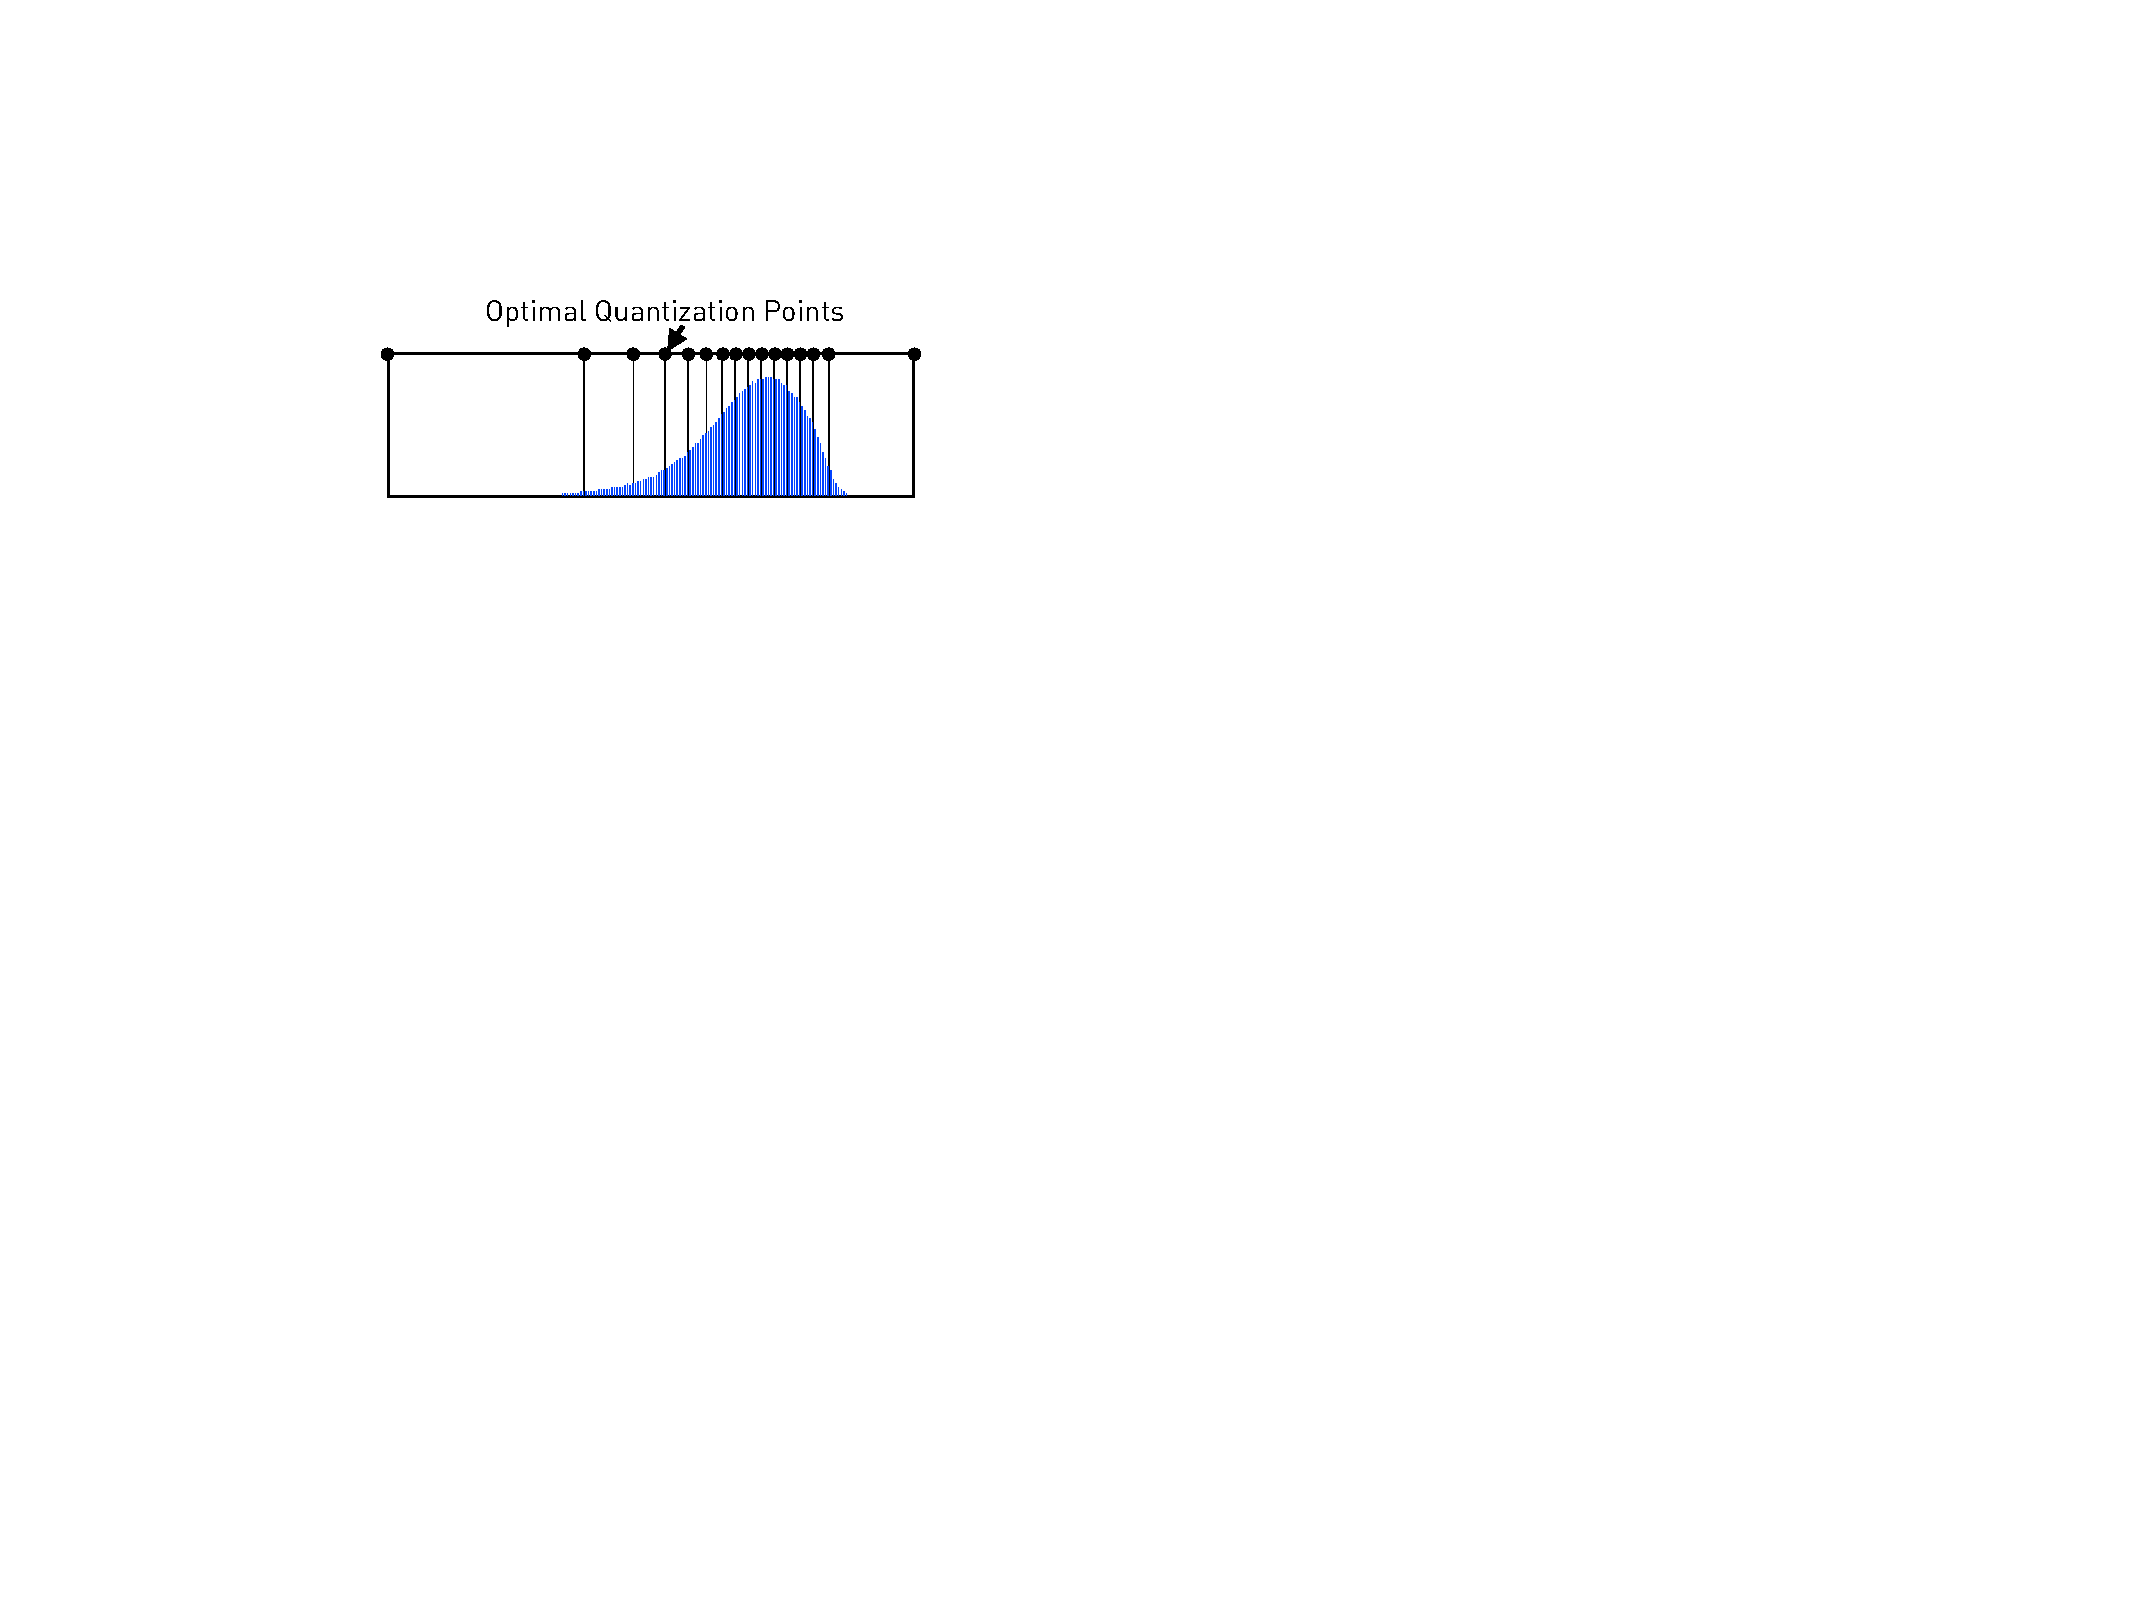
\includegraphics[width=0.5\columnwidth]{micro-experiments/dp-level.pdf} 
\vspace{-1em}
\caption{Optimal quantization points calculated with
dynamic programming given a data distribution. }
\label{fig:optimalquantization}
\end{figure} 

\vspace{-0.5em}
\paragraph*{Dynamic Programming on all $M$ candidate points}
Given $M$ candidate points, we can apply the same dynamic
programming algorithm. 
In this case,
the complexity of calculating the 
matrix $V(\cdot, \cdot)$ is $O(M^2 + N)$ and the 
complexity of calculating matrix $T(\cdot, \cdot)$ is $O(sM^2)$. The total memory cost is $O(sM + M^2)$. Note that to find the optimal quantization, we only need to scan all $N$ numbers once.
Figure~\ref{fig:optimalquantization} illlustrates
an example output for our algorithm.

\vspace{-0.5em}
\subsection{Even Faster}
\vspace{-0.5em}

We can further bring the complexity from $O(M^2)$
down to a complexity that is linear to $M$ by applying
one more layer of approximation. This algorithm is similar 
to the one given in (Acharya 431 et al., 2015) for the histogram recovery problem, although 432 the cost function 
we consider is different.
We describe the details in the full version.


%%%%

\iffalse
With this in mind, we can rephrase the problem as follows. 
Given a set of initial candidate points $\mathcal{M}$, 
let $T(k, N)$ be the optimal variance for a set of $M$ points $x_1, \ldots, x_M$, 
starting from a set of candidate points $\mathcal{M}$, using $k$ quantization levels. 
In particular, by Lemma~\ref{lem:discrete}, the original problem can be phrased as finding $T(k, N)$ given initial candidate set $\Omega$. 
In the following, we will give two different solutions to this problem: an approximate greedy algorithm, and an exact one using dynamic programming (DP). 

 \paragraph*{A Greedy Approximation Algorithm}
We now describe a nearly linear time algorithm for this problem, which we can show is provably competitive with the optimal solution.
This algorithm is similar to the one given in \cite{ADHLS15} for the histogram recovery problem, although the cost function we consider is different. 

Our algorithm, at a high level, proceeds as follows.
Suppose we wish to compete with the best quantization that uses $k$ points.
Initially, we form the partition $\setI$ so that each point in $\setX$ is in its own interval.
Then, we repeatedly do the following procedure:
\begin{enumerate}
\item
Pair up consecutive intervals in the partition, so that we form $|\setI| / 2$ ``candidate'' intervals, which we propose to merge.
For each such candidate interval $J$, compute $\err(\setX, J)$.
\item
Find the $2 k$ candidate intervals with largest $\err (\setX, J)$.
\emph{Keep} these intervals, and merge the remaining ones.
\end{enumerate}

The full pseudocode of this procedure is deferred to the full version. 
Note that each step requires only a single pass through the data. 
Moreover, we show in the full version that we can do at most $O(\log N )$ many iterations. 
Thus, the algorithm runs in $O(N \log N)$ iterations.
In the full version of the paper, we show the following guarantee on the number of remaining candidate points, and on the approximation ratio:
\begin{theorem}
\label{thm:approx}
Given any $\setX, k$, let $\setI$ be the output of the above algorithm.
Then $\setI$ has at most $4k + 1$ intervals, and we have that $\err (\setX, \setI) \leq 2 \OPT_k$.
\end{theorem}
We can tune these parameters to get a tradeoff between how many intervals remain, and how much error we tolerate. 
Theorem~\ref{thm:approx} yields a solution for $T(4k + 1, N)$ given initial candidate set $\Omega$.
Next, we define a dynamic programming solution, which can help us get a tight solution in $k$. 

%Moreover, to get the output of the algorithm down to size exactly $k$, we may also do an additional dynamic programming postprocessing routine on the output of this algorithm.
%This postprocessing now looks for the best partition with $s$ pieces at endpoints given by endpoints of $\setI$, and so runs in time $O(k^2 N)$, i.e., nearly-linear in the number of samples.


%The goal is to find  
%the optimal set of $s$ quantization 
%levels $\{l_1, l_2, \cdots, l_{s-1}\}$ 
%which minimize the mean quantization variance. Formally:
%\begin{align}
%\nonumber \min_{l_1, \cdots, l_{s-1}} \quad & \mathcal{MV}(l_1,\cdots, l_{s-1}) := {1\over N}\sum_{x\in \Omega} \sum_{k=1}^s {\bf 1}_k(x)V_k(x)\\
%\text{s.t.}\quad & 0 = l_0 \leq l_1\leq l_2 \leq \cdots \leq l_{s-1} \leq l_s = 1.
%\label{eq:opt_Q}
%\end{align}
%where ${\bf 1}_k(x)$ is the indicator function
%\[
%{\bf 1}_k(x) = 
%\begin{cases}
%1 & \text{if}~x\in (l_{k-1}, l_k] \\
%0 & \text{o.w.}
%\end{cases}
%\]
%and $V_k(x)$ is the variance function 
%\begin{align}
%V_k(x) = (x-p_{k-1})(p_k - x), \label{eq:var}
%\end{align}
%which is the variance of Bernoulli distribution with probability $l_k-x$ taking value $l_{k-1}$ and probability $x-l_{k-1}$ taking value $l_k$. ${\bf 1}_k(x)V_k(x)$ is the variance if $x$ falls into the interval $(l_{k-1}, l_k]$. 

%This problem is hard to solve directly, due to non-convexity and non-smoothness. We discretize the range $[0,1]$ into $M$ intervals, i.e., $[0,d_1), [d_1, d_2), \cdots, [d_{M-1}, 1]$ with $0< d_1<d_2<\cdots < d_{M-1}<1$. All $l_k$'s are restricted to values in $\{d_1, d_2, \cdots, d_{M-1}\}$ while satisfying  monotonicity. 
%
%\begin{theorem} \label{thm:optQ}
%Let the maximal number of data points in each ``small interval'' (defined by $\{d_m\}_{m=1}^{M-1}$) and the maximal length of small intervals be bounded by $bN/M$ and $a/M$, respectively. Let $\{l^*_k\}_{k=1}^{s-1}$ and $\{\hat{l}^*_k\}_{k=1}^{s-1}$ be the optimal quantization to \eqref{eq:opt_Q} and the solution with discretization. Let $cM/s$ be the upper bound of the number of small intervals crossed by any ``large interval'' (defined by $\{l^*_k\}_{k=1}^{s-1}$). Then we have the discretization error bounded by
%\[
% \mathcal{MV}(\hat{l}^*_1,\cdots, \hat{l}^*_{s-1}) -  \mathcal{MV}(l^*_1,\cdots, l^*_{s-1}) \leq {a^2b s \over 4 M^3} + {a^2bc^2 \over Ms}.
%\]
%\end{theorem}
%
%Note that if the numbers of data points falling into all small intervals are equal, then
%the constant $b$ is $1$. So $b$ roughly measures the uniformness of the data distribution w.r.t. small intervals. If all small intervals have equal length, then $a$ is equal to $1$. So $a$ roughly measures the distortion from equal-length small intervals. 
%Similarly, $c$ roughly measures the distortion from equal-length large intervals since $c=1$ means that all large intervals defined by $\{l^*_k\}_{k=1}^{s-1}$ roughly cross the same number of small intervals defined by $\{d_m\}_{m=1}^{M-1}$. Theorem~\ref{thm:optQ} suggests that the mean variance using the discrete variance-optimal quantization will converge to the optimal with the rate $O(1/Ms)$.


\paragraph*{Dynamic Programming}

We now describe
a dynamic programming algorithm to 
find the optimal solution given an arbitrary set of initial candidates. 
Our goal is to calculate $T(k, N)$, where $S$ is an arbitrary initial set of candidates among the points $[x_1 \ldots x_n]$. 
This problem can be solved by dynamic programing using the following recursion
\[
T(k, m) = \min_{j\in \{k-1, k, \cdots, m-1\}} T(k-1,j) + \err (\Omega, [x_j, x_m]).
\]
Notice that the term $\err (\Omega, [x_j, x_m])$ can be computed in linear time. So, the time complexity of this program is dominated by the complexity of filling in $T(\cdot, \cdot)$, which is $O(k M^2)$, where $M$ is the size of the initial candidate set $\mathcal{M}$. 
After filling in this matrix, we can find the optimal partition by classical backtracking techniques.
Figure~\ref{fig:optimalquantization} illustrates
an example output for this algorithm. 

\paragraph{Applications.} 
A natural way to combine the two algorithms is to first run the greedy approximation to get a candidate set of size $O(k)$, and then run the DP solution to obtain a tight solution in the number of intervals, using $k$ points. 
The total running time of this procedure is $O( N \log N + k^3 )$. 

Another alternative, which we employ in practice, is to first discretize the range $[0, 1]$ into $M$ intervals of uniform length, where $M$ is assumed to be a large constant, and restrict the set of initial candidates $\mathcal{M}$ to points from this set. (Notice that we can safely add points in $\mathcal{M}$ to the initial set, since their variance is $0$.) We then apply the DP approach described above to this instance of the problem. 
We obtain a solution which \emph{approximates} the optimal variance, but uses a tight set of $k$ candidates. The running time of this approach is $O( N + k M^2 )$, and bounds on its approximation guarantees are given in the supplementary material.  

\fi





%\paragraph*{Approximate dynamic programming}
%This program requires quadratic time in $N$ to run, which is often infeasible in practice.
% We discretize the range $[0,1]$ into $M$ intervals, i.e., $[0,d_1), [d_1, d_2), \cdots, [d_{M-1}, 1]$ with $0< d_1<d_2<\cdots < d_{M-1}<1$. All $l_k$'s are restricted to values in $\{d_1, d_2, \cdots, d_{M-1}\}$ while satisfying  monotonicity. 
%
%\begin{theorem} \label{thm:optQ}
%Let the maximal number of data points in each ``small interval'' (defined by $\{d_m\}_{m=1}^{M-1}$) and the maximal length of small intervals be bounded by $bN/M$ and $a/M$, respectively. Let $\{l^*_k\}_{k=1}^{s-1}$ and $\{\hat{l}^*_k\}_{k=1}^{s-1}$ be the optimal quantization to \eqref{eq:opt_Q} and the solution with discretization. Let $cM/s$ be the upper bound of the number of small intervals crossed by any ``large interval'' (defined by $\{l^*_k\}_{k=1}^{s-1}$). Then we have the discretization error bounded by
%\[
% \mathcal{MV}(\hat{l}^*_1,\cdots, \hat{l}^*_{s-1}) -  \mathcal{MV}(l^*_1,\cdots, l^*_{s-1}) \leq {a^2b s \over 4 M^3} + {a^2bc^2 \over Ms}.
%\]
%\end{theorem}
%

%where $V(j,m)$ denotes the total variance of points falling into the interval $[d_j, d_m]$. 
%The optimal value for $l_{s-1}^*$ is $ d_{j^*_{s-1}}$ with $j^*_{s-1}$ equal to
%\[
%j^*_{s-1} = \argmin_{j\in \{s-1, k, \cdots, M-1\}} T(s-1,j) + V(j,M),
%\]
%and the rest can be retrieved by 
%\begin{align*}
%j^*_{k-1} = \argmin_{j\in \{k-1, k, \cdots, j^*_k-1\}} T(k-1, j) + V(j, j^*_k) \\
%\text{for all}~k=2, \cdots, K-2
%\end{align*}

%The complexity of calculating the matrix $V(\cdot, \cdot)$ is $O(M^2 + N)$ and the complexity of calculating matrix $T(\cdot, \cdot)$ is $O(sM^2)$. The total memory cost is $O(sM + M^2)$. Note that to find the optimal quantization, we only need to scan all $N$ numbers once.
%The calculation of $V$ is not trivial (it needs
%another dynamic programming algorithm) and we
%describe the details in the full version.

%Define $T(k, m)$ be the optimal total variance for points in $[0, d_m]$ with $k$ quantization levels. Our goal is to calculate $T(s, M)$. This problem can be solved by dynamic programing using the following recursion
%\[
%T(k, m) = \min_{j\in \{k-1, k, \cdots, m-1\}} T(k-1,j) + V(j,m),
%\]
%where $V(j,m)$ denotes the total variance of points falling into the interval $[d_j, d_m]$. The optimal value for $l_{s-1}^*$ is $ d_{j^*_{s-1}}$ with $j^*_{s-1}$ equal to
%\[
%j^*_{s-1} = \argmin_{j\in \{s-1, k, \cdots, M-1\}} T(s-1,j) + V(j,M),
%\]
%and the rest can be retrieved by 
%\begin{align*}
%j^*_{k-1} = \argmin_{j\in \{k-1, k, \cdots, j^*_k-1\}} T(k-1, j) + V(j, j^*_k) \\
%\text{for all}~k=2, \cdots, K-2
%\end{align*}
%
%The complexity of calculating the matrix $V(\cdot, \cdot)$ is $O(M^2 + N)$ and the complexity of calculating matrix $T(\cdot, \cdot)$ is $O(sM^2)$. The total memory cost is $O(sM + M^2)$. Note that to find the optimal quantization, we only need to scan all $N$ numbers once.
%The calculation of $V$ is not trivial (it needs
%another dynamic programming algorithm) and we
%describe the details in the full version.
%Figure~\ref{fig:optimalquantization} illlustrates
%an example output for our algorithm.


\iffalse
\begin{proof}
Let $p^*_0$ be $0$ and $p^*_K=1$.We quantitize $\{p^*_k\}_{k=1}^{K-1}$ one element by one element, while monitor the changing of the total variance $N \times \mathcal{MV(\cdot)}$. We first quantize $p^*_1$ to the closest value (denoted it by $Q(p^*_1)$) in $\{d_m\}_{m=1}^{M-1} \cup \{p^*_0,p^*_K\}$ under the monotonicity constraint, that is, $p^*_0\leq Q(p^*_1) \leq p^*_2$. Here, one important observation is $|p^*_{1} - Q(p^*_1)|\leq a/M$. Consider the total variance of this new solution $Q(p^*_1), p^*_2, \cdots, p^*_{K-1}$. The variance of points falling into the range $[p^*_2, 1]$ does not change at all. Without the loss of generality, assume $p^*_{1} \geq Q(p^*_1)$.

Next we consider points falling into the following three sets $C_1 = [p^*_0, Q(p^*_1)]$, $C_2 = [Q(p^*_1), p^*_1]$, and $C_3 = [p^*_1, p^*_2]$. The variance of points of falling into $C_1$ gets reduced from the form of variance in \eqref{eq:var}. Next we only need to check the variance change for points in $C_2$ and $C_3$. Consider $C_2$ first. The variance for point $x$ in $C_2$ is
\[
(x-Q(p^*_1))(p^*_1 - x) \leq {a^2 \over 4 M^2}. 
\]  
Thus, the change of variance for points in $C_2$ would be bounded by ${a^2 \over 4 M^2}$. Then consider $C_3$. The change of variance for point $x$ in $C_3$ is
\begin{align*}
& (x-Q(p^*_1))(p^*_2 - x) - (x-p^*_1) (p^*_2 - x) 
\\
= & (p^*_1 - Q(p^*_1)) (p^*_2 - x)
\\
\leq & {a\over M}(p^*_2 - x)
\end{align*}
Therefore, the change of total variance from $\{p^*_1, p^*_2, \cdots, p^*_{K-1}\}$ to $\{Q(p^*_1), p^*_2, \cdots, p^*_{K-1}\}$ is bounded by 
\begin{align}
\nonumber
& \sum_{x\in C_2} {a^2 \over 4M^2} + \sum_{x \in C_3} {a\over M}(p^*_2 - x)
\\
\nonumber
\leq & {Nb \over M} {a^2 \over 4M^2} + {a\over M}{Nb \over M} \sum_{t=1}^{cM/K}t{a\over M}
\\
\leq &
{a^2b N \over 4 M^3} + {a^2bc^2 N \over MK^2}
\label{eq:bound_1step}
\end{align}
Similarly, we quantitize $p^2_2$ in $\{Q(p^*_1), p^*_2, \cdots, p^*_{K-1}\}$ to get a new solution $\{Q(p^*_1), Q(p^*_2), \cdots, p^*_{K-1}\}$ while maintain the monotonicity. We can establish the same upper bound to \eqref{eq:bound_1step}. Following this idea, we can obtain a quantization solution $\{Q(p^*_1), Q(p^*_2), \cdots, Q(p^*_{K-1})\}$. Therefore, we obtain that 
\begin{align*}
&  \mathcal{MV}(Q(p^*_1), Q(p^*_2), \cdots, Q(p^*_{K-1})) -  \mathcal{MV}({p}^*_1,\cdots, {p}^*_{K-1}) 
 \\
 & \quad \leq {a^2b K \over 4 M^3} + {a^2bc^2 \over MK}.
\end{align*}
Using the fact that $ \mathcal{MV}(p^*_1,\cdots, p^*_{K-1})$ is smaller than $\mathcal{MV}(Q(p^*_1), Q(p^*_2), \cdots, Q(p^*_{K-1}))$ proves the claim.
\end{proof}


\paragraph*{A Greedy Approximation Algorithm}
We now describe a nearly linear time algorithm for this problem, which we can show is provably competitive with the optimal solution.
This algorithm is very similar to one by \cite{ADHLS15} for the histogram recovery problem.

Our algorithm, at a high level, proceeds as follows.
Suppose we wish to compete with the best quantization that uses $k$ points.
Initially, we form the partition $\setI$ so that each point in $\setX$ is in its own interval.
Then, we repeatedly do the following procedure:
\begin{enumerate}
\item
Pair up consecutive intervals in the partition, so that we form $|\setI| / 2$ ``candidate'' intervals, which we propose to merge.
For each such candidate interval $J$, compute $\err(\setX, J)$.
\item
Find the $2 s$ candidate intervals with largest $\err (\setX, J)$.
Do not merge these intervals, and merge the remaining.
\end{enumerate}

We defer the formal pseudocode of this to the full version.
Each step requires only a single pass through the data.
Moreover, we show in the full version that we can do at most logarithmically many iterations.
Thus, the algorithm runs in nearly linear time.
In the full version of the paper, we show:
\begin{theorem}
Given any $\setX, k$, let $\setI$ be the output of the above algorithm.
Then $\setI$ has at most $4s + 1$ intervals, and we have that $\err (\setX, \setI) \leq 2 \OPT_s$.
\end{theorem}
We can tune these parameters, to get a tradeoff between how many intervals remain, and how much error we tolerate.
Moreover, to get the output of the algorithm down to size exactly $s$, we may also do an additional dynamic programming postprocessing routine on the output of this algorithm.
This postprocessing now looks for the best partition with $s$ pieces at endpoints given by endpoints of $\setI$, and so runs in time $O(s^2 N)$, i.e., nearly-linear in the number of samples.
\fi

%We require the following lemma, whose proof is trivial and omitted.
%\begin{lemma}
%If $I \subseteq I'$, then $\err(\setX, I) = \err (\setX_I, I) \leq \err (\setX_I, I')$.
%\end{lemma}









